\documentclass[t]{beamer}
\usepackage{mathtools}
\usepackage{tikz}
\usepackage{pgfplots}
\usepackage{ulem}
\usetikzlibrary{arrows,backgrounds,shapes,matrix,positioning,fit}
\newcommand{\argmax}{\operatornamewithlimits{argmax}}
\newcommand{\argmin}{\operatornamewithlimits{argmin}}
\newcommand{\wt}{\operatornamewithlimits{wt}}
\newcommand{\var}{\operatornamewithlimits{var}}
\renewcommand\Re{\operatorname{Re}}
\renewcommand\Im{\operatorname{Im}}

\mode<presentation>
{
  \usetheme{Singapore}
  %\useoutertheme{infolines} % Showing only current section in navigation
  \setbeamertemplate{headline}{}  % Empty headline
  \setbeamertemplate{footline}[frame number]  % Getting rid of footer items except slide number
  \setbeamercovered{invisible}
  \beamertemplatenavigationsymbolsempty % Getting rid of navigation bullets at the bottom
}
\usepackage[english]{babel}
\usepackage[latin1]{inputenc}
\usepackage{times}
\usepackage[T1]{fontenc}

\title[EE 703 DMT]{Performance of ML Receiver for $M$-ary Signaling}
\author[Saravanan V]
{
  Saravanan Vijayakumaran\\
  \href{mailto:sarva@ee.iitb.ac.in}{sarva@ee.iitb.ac.in}
}
\institute[IIT Bombay]
{
  Department of Electrical Engineering\\
  Indian Institute of Technology Bombay
}
\date{October 8, 2013}

\AtBeginSection[]%
{%
\begin{frame}[plain]%
  \topskip0pt
  \vspace*{\fill}
    \begin{center}%
      \usebeamerfont{section title}\insertsection%
    \end{center}%
  \vspace*{\fill}
\end{frame}%
}

\begin{document}

\begin{frame}
  \titlepage
\end{frame}

\section{Performance of ML Decision Rule for $M$-ary signaling}
%% Frame %%
\begin{frame}{ML Decision Rule for $M$-ary Signaling}
  \footnotesize
  \begin{itemize}
    \item \pause $M$ equally likely hypotheses
      \begin{equation*}
        \begin{array}{ccc}
            H_1 & : & y(t) = s_1(t) + n(t) \\
            H_2 & : & y(t) = s_2(t) + n(t) \\
            \vdots &   &  \vdots          \\
            H_M & : & y(t) = s_M(t) + n(t) \\
        \end{array}
      \end{equation*}
    \item \pause The ML decision rule for real AWGN channel is
      \begin{eqnarray*}
        \delta_{ML}(y) = \argmin_{1 \leq i \leq M} \lVert y - s_i \rVert^2 = \argmax_{1 \leq i \leq M} \langle y, s_i \rangle - \frac{\lVert s_i \rVert^2}{2}
      \end{eqnarray*}
    \item \pause The ML decision rule for complex AWGN channel is
      \begin{eqnarray*}
        \delta_{ML}(y) = \argmin_{1 \leq i \leq M} \lVert y - s_i \rVert^2 = \argmax_{1 \leq i \leq M} \Re\left(\langle y, s_i \rangle\right) - \frac{\lVert s_i \rVert^2}{2}
      \end{eqnarray*}
    \item \pause In general, there is no neat expression for $P_e$ as in the binary case
  \end{itemize}
  \normalsize
\end{frame}

%% Frame %%
\begin{frame}{QPSK}
  \footnotesize
  \begin{itemize}
    \item \pause QPSK signals where $p(t)$ is a real baseband pulse of duration $T$
    \begin{eqnarray*}
      s_1^p(t) & = & \sqrt{2}p(t)\cos \left( 2\pi f_c t + \frac{\pi}{4}\right) \\ \pause
      s_2^p(t) & = & \sqrt{2}p(t)\cos \left( 2\pi f_c t + \frac{3\pi}{4}\right) \\ \pause
      s_3^p(t) & = & \sqrt{2}p(t)\cos \left( 2\pi f_c t + \frac{5\pi}{4}\right) \\ \pause
      s_4^p(t) & = & \sqrt{2}p(t)\cos \left( 2\pi f_c t + \frac{7\pi}{4}\right)
    \end{eqnarray*}
    \item \pause Complex envelopes of QPSK Signals
      \begin{eqnarray*}
        s_1(t) = p(t)e^{\ j\frac{\pi}{4}}, \pause
        s_2(t) = p(t)e^{\ j\frac{3\pi}{4}}, \pause
        s_3(t) = p(t)e^{\ j\frac{5\pi}{4}}, \pause
        s_4(t) = p(t)e^{\ j\frac{7\pi}{4}}
      \end{eqnarray*}
    \item \pause Orthonormal basis for the complex envelopes consists of \pause only
      \begin{equation*}
        \phi(t) = \frac{p(t)}{\sqrt{E_p}}
      \end{equation*}
  \end{itemize}
  \normalsize
\end{frame}

%% Frame %%
\begin{frame}{ML Receiver for QPSK}
  \footnotesize
  \begin{itemize}
    \item \pause $E_b = \pause E_p/2$
    \item \pause The vector representation of the QPSK signals is
      \begin{eqnarray*}
        s_1 & = &  \sqrt{E_b} + j\sqrt{E_b} \\ \pause
        s_2 & = & -\sqrt{E_b} + j\sqrt{E_b} \\ \pause
        s_3 & = & -\sqrt{E_b} - j\sqrt{E_b} \\ \pause
        s_4 & = &  \sqrt{E_b} - j\sqrt{E_b} 
      \end{eqnarray*}
    \item \pause The hypothesis testing problem in terms of vectors is
      \begin{equation*}
        H_i  :  Y = s_i + N, \ \ i=1,\ldots,4
      \end{equation*}
      \pause where  $N \sim \mathcal{CN}(0, 2\sigma^2)$
    \item \pause The ML decision rule is given by
      \begin{eqnarray*}
        \delta_{ML}(y) = \pause \argmin_{1 \leq i \leq 4} \lVert y - s_i \rVert^2 = \argmax_{1 \leq i \leq 4} \Re\left(\langle y, s_i \rangle\right) - \frac{\lVert s_i \rVert^2}{2}
      \end{eqnarray*}
    \item \pause The ML decision rule decides $s_i$ was transmitted if $y$ belongs to the $i$th quadrant
  \end{itemize}
  \normalsize
\end{frame}

%% Frame %%
\begin{frame}{ML Decision Rule for QPSK}
  \footnotesize
  \begin{figure}
    \centering
      \begin{tikzpicture}[scale=0.8,transform shape]
        \begin{axis}[
                     xmax=1.5,
                     xmin=-1.5,
                     ymax=1.5,
                     ymin=-1.5,
                     axis lines = middle,
                     ytick={1.45},
                     yticklabels = {$Y_s$},
                     xtick={1.46},
                     xticklabels = {$Y_c$},
                     x post scale = 1.0,
                     xticklabel shift = -20pt,
                     %y axis line style={-},
                     %x axis line style={-},
                     nodes near coords,
                    ]
          \addplot+[only marks, 
                    mark options={draw=black,fill=black},
                    point meta=explicit symbolic
                    ] 
                    coordinates {
                      (1,1)[$(\sqrt{E_b},\sqrt{E_b})$] 
                      (-1,1)[$(-\sqrt{E_b},\sqrt{E_b})$] 
                      (-1,-1)[$(-\sqrt{E_b},-\sqrt{E_b})$] 
                      (1,-1)[$(\sqrt{E_b},-\sqrt{E_b})$]
                    };
        \end{axis}
      \end{tikzpicture}
  \end{figure}
  \begin{eqnarray*}
    \pause P_{e|1}  =  \pause \Pr\left[ Y_c < 0 \text{ or } Y_s < 0 \bigg| (\sqrt{E_b}, \sqrt{E_b}) \text{ was sent} \right] 
  \end{eqnarray*}
  \normalsize
\end{frame}

%% Frame %%
\begin{frame}{ML Decision Rule for QPSK}
  \footnotesize
  \begin{itemize}
    \item \pause Probability of error when $s_1$ is transmitted is
      \begin{eqnarray*}
        P_{e|1} & = & \pause \Pr\left[ Y_c < 0 \text{ or } Y_s < 0 \bigg| (\sqrt{E_b}, \sqrt{E_b}) \text{ was sent} \right] \\
                & = & \pause 2Q\left(\sqrt{\frac{2E_b}{N_0} }\right) -Q^2\left(\sqrt{\frac{2E_b}{N_0} }\right) 
      \end{eqnarray*}
    \item \pause By symmetry, 
      \begin{eqnarray*}
        P_{e|1} = P_{e|2} = P_{e|3} = P_{e|4}
      \end{eqnarray*}
    \item \pause The average probability of error is
      \begin{eqnarray*}
        P_{e} = \frac{1}{4} \sum_{i=1}^4 P_{e|i} \pause = P_{e|1} =  \pause 2Q\left(\sqrt{\frac{2E_b}{N_0} }\right) -Q^2\left(\sqrt{\frac{2E_b}{N_0} }\right) 
      \end{eqnarray*}
  \end{itemize}
  \normalsize
\end{frame}

%% Frame %%
\begin{frame}{ML Decision Rule for 16-QAM}
  \footnotesize
  \begin{figure}
    \centering
      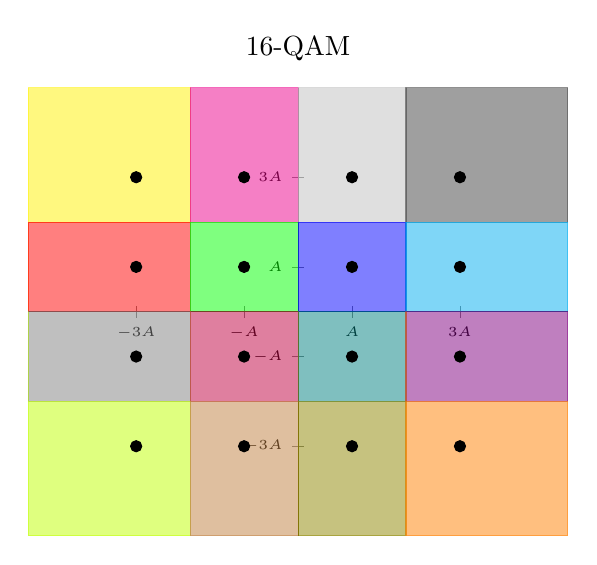
\begin{tikzpicture}[scale=1.0,transform shape]
        \begin{axis}[
                     title={16-QAM},
                     xmax=5,
                     xmin=-5,
                     ymax=5,
                     ymin=-5,
                     axis lines = middle,
                     xtick = {-3, -1, 1, 3},
                     xticklabels = {$-3A$, $-A$, $A$, $3A$},
                     x tick label style = {font = \tiny},
                     ytick = {-3, -1, 1, 3},
                     yticklabels = {$-3A$, $-A$, $A$, $3A$},
                     y tick label style = {font = \tiny},
                     y axis line style={-},
                     x axis line style={-},
                    ]
          \addplot+[only marks, 
                    mark options={draw=black,fill=black},
                    ] 
                    coordinates {
                      (3,1)
                      (1,3)
                      (-1,3)
                      (-3,1)
                      (-3,-1)
                      (-1,-3)
                      (1,-3)
                      (3,-1)
                      (1,1)
                      (-1,1)
                      (1,-1)
                      (-1,-1)
                      (3,3)
                      (-3,3)
                      (3,-3)
                      (-3,-3)
                    };
        \addplot[color=yellow,fill=yellow,opacity=0.5] coordinates {(-5,2) (-2,2) (-2,5) (-5,5)} \closedcycle;
        \addplot[color=magenta,fill=magenta,opacity=0.5] coordinates {(-2,2) (0,2) (0,5) (-2,5)} \closedcycle;
        \addplot[color=lightgray,fill=lightgray,opacity=0.5] coordinates {(0,2) (2,2) (2,5) (0,5)} \closedcycle;
        \addplot[color=darkgray,fill=darkgray,opacity=0.5] coordinates {(2,2) (5,2) (5,5) (2,5)} \closedcycle;
        \addplot[color=red,fill=red,opacity=0.5] coordinates {(-5,0) (-2,0) (-2,2) (-5,2)} \closedcycle;
        \addplot[color=green,fill=green,opacity=0.5] coordinates {(-2,0) (0,0) (0,2) (-2,2)} \closedcycle;
        \addplot[color=blue,fill=blue,opacity=0.5] coordinates {(0,0) (2,0) (2,2) (0,2)} \closedcycle;
        \addplot[color=cyan,fill=cyan,opacity=0.5] coordinates {(2,0) (5,0) (5,2) (2,2)} \closedcycle;
        \addplot[color=gray,fill=gray,opacity=0.5] coordinates {(-5,-2) (-2,-2) (-2,0) (-5,0)} \closedcycle;
        \addplot[color=purple,fill=purple,opacity=0.5] coordinates {(-2,-2) (0,-2) (0,0) (-2,0)} \closedcycle;
        \addplot[color=teal,fill=teal,opacity=0.5] coordinates {(0,-2) (2,-2) (2,0) (0,0)} \closedcycle;
        \addplot[color=violet,fill=violet,opacity=0.5] coordinates {(2,-2) (5,-2) (5,0) (2,0)} \closedcycle;
        \addplot[color=lime,fill=lime,opacity=0.5] coordinates {(-5,-5) (-2,-5) (-2,-2) (-5,-2)} \closedcycle;
        \addplot[color=brown,fill=brown,opacity=0.5] coordinates {(-2,-5) (0,-5) (0,-2) (-2,-2)} \closedcycle;
        \addplot[color=olive,fill=olive,opacity=0.5] coordinates {(0,-5) (2,-5) (2,-2) (0,-2)} \closedcycle;
        \addplot[color=orange,fill=orange,opacity=0.5] coordinates {(2,-5) (5,-5) (5,-2) (2,-2)} \closedcycle;
        \end{axis}
      \end{tikzpicture}
  \end{figure}
  \pause Exact analysis is tedious. \pause Approximate analysis is sufficient.
  \normalsize
\end{frame}

\section{Revisiting the $Q$ function}
%% Frame %%
\begin{frame}{Revisiting the $Q$ function}
  \footnotesize
  $X \sim N(0,1)$
  \begin{equation*}
    Q(x) = P\left[X > x \right] = \int_{x}^{\infty} \frac{1}{\sqrt{2\pi}} \exp{\left(\frac{-t^2}{2}\right)} \ dt
  \end{equation*}
  \pause
  \begin{figure}
    \centering
      \begin{tikzpicture}[scale=0.55,transform shape]
        \begin{axis}[
                     title=$p(t)$,
                     xmax=5.9,
                     xmin=-5.9,
                     ymax=0.3,
                     ymin=-0.01,
                     axis lines = middle,
                     xtick = {1,5.8},
                     xticklabels = {$x$,$t$},
                     ytick=\empty,
                     x post scale = 2.0
                    ]
              \addplot[color=blue,fill=blue,fill opacity=0.5,area legend, very thick,domain=1:6,samples=100] gnuplot{exp(-x*x/(2*2))/sqrt(2*pi*2)} \closedcycle;
              \addlegendentry{$Q(x)$}
              \addplot[color=red,fill=red,fill opacity=0.5,area legend, very thick,domain=-6:1,samples=100] gnuplot{exp(-x*x/(2*2))/sqrt(2*pi*2)} \closedcycle;
              \addlegendentry{$\Phi(x)$}

        \end{axis}
      \end{tikzpicture}
  \end{figure}
  \normalsize
\end{frame}

%% Frame %%
\begin{frame}{Bounds on $Q(x)$ for Large Arguments}
  \footnotesize
  \begin{figure}
    \centering
      \begin{tikzpicture}[scale=0.75,transform shape]
        \begin{semilogyaxis}[
                     xlabel=$x$,
                     xmax=5,
                     xmin=0,
                     ymax=1,
                     ymin=1e-8,
                     x post scale = 1.5
                    ]
          \addplot[smooth, thick, black]gnuplot{0.5*erfc((x/sqrt(2)))};
          \addlegendentry{$Q(x)$}
          \addplot[smooth, thick, red, domain=0.1:5, samples=100]gnuplot{(exp(-(x*x)/2))/(x*sqrt(2*pi))};
          \addlegendentry{UB in (\ref{eqn:Qbounds})}
          \addplot[smooth, thick, blue, domain=1:5, samples=100]gnuplot{(1-1/(x*x))*(exp(-(x*x)/2))/(x*sqrt(2*pi))};
          \addlegendentry{LB in (\ref{eqn:Qbounds})}
        \end{semilogyaxis}
      \end{tikzpicture}
  \end{figure}
  \begin{equation}
    \left(1 - \frac{1}{x^2} \right) \frac{e^{-\frac{x^2}{2}}}{x\sqrt{2\pi}} \leq Q(x) \leq \frac{e^{-\frac{x^2}{2}}}{x\sqrt{2\pi}}
    \label{eqn:Qbounds}
  \end{equation}
  \normalsize
\end{frame}

%% Frame %%
\begin{frame}{$Q$ Functions with Smallest Arguments Dominate}
  \footnotesize
  \begin{figure}
    \centering
      \begin{tikzpicture}[scale=0.75,transform shape]
        \begin{semilogyaxis}[
                     xlabel=$x$,
                     xmax=3,
                     xmin=0,
                     ymax=1,
                     ymin=1e-3,
                     x post scale = 1.5
                    ]
          \addplot[smooth, thick, blue]gnuplot{0.5*erfc((x/sqrt(2)))};
          \addlegendentry{$Q(x)$}
          \addplot[smooth, thick, red]gnuplot{0.5*erfc(2*x/sqrt(2)) +  0.5*erfc((x/sqrt(2)))};
          \addlegendentry{$Q(x) + Q(2x)$}
          \addplot[smooth, thick, black]gnuplot{0.5*erfc(x/sqrt(2)) +  0.5*erfc((2*x/sqrt(2))) + 0.5*erfc(3*x/sqrt(2))};
          \addlegendentry{$Q(x) + Q(2x) +  Q(3x)$}
        \end{semilogyaxis}
      \end{tikzpicture}
  \end{figure}
  \begin{itemize}
    \item \pause $P_e$ in AWGN channels can be bounded by a sum of $Q$ functions
    \item \pause The $Q$ function with the smallest argument is used to approximate $P_e$
  \end{itemize}
  \normalsize
\end{frame}

\section{Union Bound}
%% Frame %%
\begin{frame}{Union Bound for $M$-ary Signaling in AWGN}
  \footnotesize
  \begin{itemize}
    \item \pause Let $Z_i$ be $\langle y, s_i \rangle - \frac{\lVert s_i \rVert^2}{2}$or $\Re\left(\langle y, s_i \rangle\right) - \frac{\lVert s_i \rVert^2}{2}$
    \item \pause The conditional error probability given $H_i$ is true is
      \begin{equation*}
        P_{e|i} = \Pr\left[\bigcup_{j \neq i} \left\{ Z_i < Z_j \right\} \bigg| H_i \right]
      \end{equation*}
    \item \pause Since $P(A \cup B) \leq P(A) + P(B)$, we have
      \begin{equation*}
        P_{e|i} \leq \pause \sum_{j \neq i} \Pr\left[Z_i < Z_j \bigg| H_i \right] \pause = \sum_{j \neq i} Q\left( \frac{\lVert s_j - s_i \rVert}{2\sigma} \right)
      \end{equation*}
    \item \pause The error probability is given by
      \begin{equation*}
        P_{e} = \frac{1}{M} \sum_{i=1}^M P_{e|i}  \leq \frac{1}{M}\sum_{i=1}^M \sum_{j \neq i} Q\left( \frac{\lVert s_j - s_i \rVert}{2\sigma} \right)
      \end{equation*}
  \end{itemize}
  \normalsize
\end{frame}

%% Frame %%
\begin{frame}{Union Bound for QPSK}
  \footnotesize
  \begin{figure}
    \centering
      \begin{tikzpicture}[scale=0.6,transform shape]
        \begin{axis}[
                     xmax=1.5,
                     xmin=-1.5,
                     ymax=1.5,
                     ymin=-1.5,
                     axis lines = middle,
                     ytick={1.45},
                     yticklabels = {$Y_s$},
                     xtick={1.46},
                     xticklabels = {$Y_c$},
                     x post scale = 1.0,
                     xticklabel shift = -20pt,
                     nodes near coords,
                    ]
          \addplot+[only marks, 
                    mark options={draw=black,fill=black},
                    point meta=explicit symbolic
                    ] 
                    coordinates {
                      (1,1)[$s_1$]
                      (-1,1)[$s_2$]
                      (-1,-1)[$s_3$]
                      (1,-1)[$s_4$]
                    };
        \end{axis}
      \end{tikzpicture}
  \end{figure}
  \begin{eqnarray*}
    P_{e|1} & = & \pause \Pr\left[\cup_{j \neq 1} \left\{ Z_1 < Z_j \right\} \bigg| H_1 \right] \pause \leq \sum_{j \neq 1} \Pr\left[Z_1 < Z_j \bigg| H_1 \right] \\ \pause
    P_{e|1} & \leq & Q\left( \frac{\lVert s_2 - s_1\rVert}{2\sigma}\right) + Q\left( \frac{\lVert s_3 - s_1\rVert}{2\sigma}\right) + Q\left( \frac{\lVert s_4 - s_1\rVert}{2\sigma}\right) \\
            & = & \pause 2Q\left(\sqrt{\frac{2E_b}{N_0} }\right) +Q\left(\sqrt{\frac{4E_b}{N_0} }\right) 
  \end{eqnarray*}
  \normalsize
\end{frame}

%% Frame %%
\begin{frame}{Union Bound for QPSK}
  \footnotesize
  \begin{itemize}
    \item Union bound on error probability of ML rule
      \begin{equation*}
        P_e  \leq  \pause 2Q\left(\sqrt{\frac{2E_b}{N_0} }\right) +Q\left(\sqrt{\frac{4E_b}{N_0} }\right) 
      \end{equation*}
    \item \pause Exact error probability of ML rule
      \begin{equation*}
        P_{e} = 2Q\left(\sqrt{\frac{2E_b}{N_0} }\right) -Q^2\left(\sqrt{\frac{2E_b}{N_0} }\right) 
      \end{equation*}
  \end{itemize}
  \normalsize
\end{frame}

%% Frame %%
\begin{frame}{Union Bound and Exact Error Probability for QPSK}
  \footnotesize
  \begin{figure}
    \centering
      \begin{tikzpicture}[scale=0.9,transform shape]
        \begin{semilogyaxis}[
                     xlabel=$x$,
                     xmax=3,
                     xmin=0,
                     ymax=1,
                     ymin=1e-3,
                     x post scale = 1.5
                    ]
          \addplot[smooth, thick, red]gnuplot{erfc(sqrt(2)*x/sqrt(2)) +  0.5*erfc((2*x/sqrt(2)))};
          \addlegendentry{Union Bound}
          \addplot[smooth, thick, black]gnuplot{erfc(sqrt(2)*x/sqrt(2)) - 0.5*erfc((sqrt(2)*x/sqrt(2)))*0.5*erfc((sqrt(2)*x/sqrt(2)))};
          \addlegendentry{$P_e$}
        \end{semilogyaxis}
      \end{tikzpicture}
  \end{figure}
  \normalsize
\end{frame}

\section{Intelligent Union Bound}
%% Frame %%
\begin{frame}{QPSK Error Events}
  \footnotesize
  \begin{eqnarray*}
    E_1  =  \pause \left[ Z_2 > Z_1 \right] \cup \left[ Z_3 > Z_1 \right] \cup \left[ Z_4 > Z_1 \right]  \only<7>{= \left[ Z_2 > Z_1 \right] \cup \left[ Z_4 > Z_1 \right] }\pause 
  \end{eqnarray*}
  \begin{figure}
    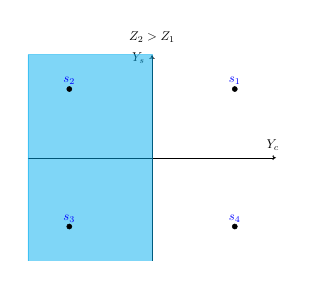
\begin{tikzpicture}[scale=0.46,transform shape]
      \begin{axis}[
                   title={$Z_2 > Z_1$},
                   xmax=1.5,
                   xmin=-1.5,
                   ymax=1.5,
                   ymin=-1.5,
                   axis lines = middle,
                   ytick={1.45},
                   yticklabels = {$Y_s$},
                   xtick={1.46},
                   xticklabels = {$Y_c$},
                   x post scale = 1.0,
                   xticklabel shift = -20pt,
                  ]
        \addplot+[only marks, 
                  nodes near coords,
                  mark options={draw=black,fill=black},
                  point meta=explicit symbolic
                  ] 
                  coordinates {
                    (1,1)[$s_1$]
                    (-1,1)[$s_2$]
                    (-1,-1)[$s_3$]
                    (1,-1)[$s_4$]
                  };
        \addplot[color=cyan,fill=cyan,opacity=0.5] coordinates {(-1.5,1.5) (-1.5,-1.5) (0,-1.5) (0,1.5) (-1.5,1.5)} \closedcycle;
      \end{axis}
    \end{tikzpicture}
    \pause
    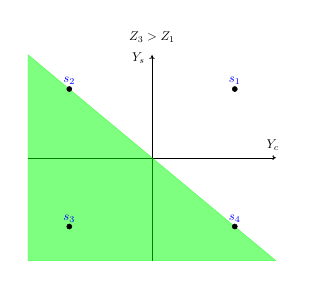
\begin{tikzpicture}[scale=0.46,transform shape]
      \begin{axis}[
                   title={$Z_3 > Z_1$},
                   xmax=1.5,
                   xmin=-1.5,
                   ymax=1.5,
                   ymin=-1.5,
                   axis lines = middle,
                   ytick={1.45},
                   yticklabels = {$Y_s$},
                   xtick={1.46},
                   xticklabels = {$Y_c$},
                   x post scale = 1.0,
                   xticklabel shift = -20pt,
                  ]
        \addplot+[only marks, 
                  nodes near coords,
                  mark options={draw=black,fill=black},
                  point meta=explicit symbolic
                  ] 
                  coordinates {
                    (1,1)[$s_1$]
                    (-1,1)[$s_2$]
                    (-1,-1)[$s_3$]
                    (1,-1)[$s_4$]
                  };
        \addplot[color=green,fill=green,opacity=0.5] coordinates {(-1.5,1.5) (-1.5,-1.5) (1.5,-1.5) (-1.5,1.5)} \closedcycle;
      \end{axis}
    \end{tikzpicture}
    \pause
    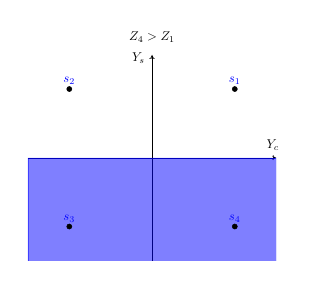
\begin{tikzpicture}[scale=0.46,transform shape]
      \begin{axis}[
                   title={$Z_4 > Z_1$},
                   xmax=1.5,
                   xmin=-1.5,
                   ymax=1.5,
                   ymin=-1.5,
                   axis lines = middle,
                   ytick={1.45},
                   yticklabels = {$Y_s$},
                   xtick={1.46},
                   xticklabels = {$Y_c$},
                   x post scale = 1.0,
                   xticklabel shift = -20pt,
                  ]
        \addplot+[only marks, 
                  nodes near coords,
                  mark options={draw=black,fill=black},
                  point meta=explicit symbolic
                  ] 
                  coordinates {
                    (1,1)[$s_1$]
                    (-1,1)[$s_2$]
                    (-1,-1)[$s_3$]
                    (1,-1)[$s_4$]
                  };
        \addplot[color=blue,fill=blue,opacity=0.5] coordinates {(-1.5,0) (-1.5,-1.5) (1.5,-1.5) (1.5,0)} \closedcycle;
      \end{axis}
    \end{tikzpicture}
    \pause
    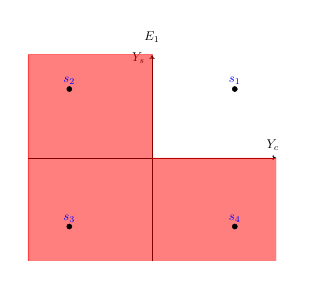
\begin{tikzpicture}[scale=0.46,transform shape]
      \begin{axis}[
                   title={$E_1$},
                   xmax=1.5,
                   xmin=-1.5,
                   ymax=1.5,
                   ymin=-1.5,
                   axis lines = middle,
                   ytick={1.45},
                   yticklabels = {$Y_s$},
                   xtick={1.46},
                   xticklabels = {$Y_c$},
                   x post scale = 1.0,
                   xticklabel shift = -20pt,
                  ]
        \addplot+[only marks, 
                  nodes near coords,
                  mark options={draw=black,fill=black},
                  point meta=explicit symbolic
                  ] 
                  coordinates {
                    (1,1)[$s_1$]
                    (-1,1)[$s_2$]
                    (-1,-1)[$s_3$]
                    (1,-1)[$s_4$]
                  };
        \addplot[color=red,fill=red,opacity=0.5] coordinates {(-1.5,1.5) (-1.5,-1.5) (1.5,-1.5) (1.5,0) (0,0) (0,1.5) (-1.5,1.5)} \closedcycle;
      \end{axis}
    \end{tikzpicture}
    \pause
  \end{figure}
  \normalsize
\end{frame}

%% Frame %%
\begin{frame}{Intelligent Union Bound for QPSK}
  \footnotesize
  \begin{itemize}
    \item \pause Intelligent union bound on $P_{e|1}$
      \begin{eqnarray*}
        P_{e|1} & = & \pause \Pr\left[\left( Z_2 > Z_1 \right) \cup \left( Z_4 > Z_1 \right) \bigg| H_1 \right] \\ \pause
                & \leq & \Pr\left[Z_2 > Z_1 \bigg| H_1 \right] + \Pr\left[Z_4 > Z_1 \bigg| H_1 \right]\\ \pause
                & = & Q\left( \frac{\lVert s_2 - s_1\rVert}{2\sigma}\right) + Q\left( \frac{\lVert s_4 - s_1\rVert}{2\sigma}\right) \\
                & = & \pause 2Q\left(\sqrt{\frac{2E_b}{N_0} }\right)
      \end{eqnarray*}
    \item By symmetry $P_{e|1} = P_{e|2} = P_{e|3} = P_{e|4}$ and
      \begin{eqnarray*}
        P_e \leq \pause 2Q\left(\sqrt{\frac{2E_b}{N_0} }\right)
      \end{eqnarray*}
  \end{itemize}
  \normalsize
\end{frame}

%% Frame %%
\begin{frame}{Intelligent Union Bound and Exact Error Probability for QPSK}
  \footnotesize
  \begin{figure}
    \centering
      \begin{tikzpicture}[scale=0.9,transform shape]
        \begin{semilogyaxis}[
                     xlabel=$x$,
                     xmax=3,
                     xmin=0,
                     ymax=1,
                     ymin=1e-3,
                     x post scale = 1.5
                    ]
          \addplot[smooth, thick, blue]gnuplot{erfc(sqrt(2)*x/sqrt(2)) +  0.5*erfc((2*x/sqrt(2)))};
          \addlegendentry{Union Bound}
          \addplot[smooth, thick, red]gnuplot{erfc(sqrt(2)*x/sqrt(2))};
          \addlegendentry{Int Union Bound}
          \addplot[smooth, thick, black]gnuplot{erfc(sqrt(2)*x/sqrt(2)) - 0.5*erfc((sqrt(2)*x/sqrt(2)))*0.5*erfc((sqrt(2)*x/sqrt(2)))};
          \addlegendentry{$P_e$}
        \end{semilogyaxis}
      \end{tikzpicture}
  \end{figure}
  \normalsize
\end{frame}

%% Frame %%
\begin{frame}{General Strategy for Intelligent Union Bound}
  \footnotesize
  \begin{itemize}
    \item \pause Let $N_{ML}(i)$ be the smallest set of neighbors of $s_i$ which define the decision region $\Gamma_i$
      \begin{eqnarray*}
        \Gamma_i = \left\{y \bigg| \delta_{ML}(y) = i\right\} = \pause \left\{y \bigg| Z_i \geq Z_j \text{ for all } j \in N_{ML}(i)\right\}
      \end{eqnarray*}
    \item \pause Probability of error when $s_i$ is transmitted is
      \begin{eqnarray*}
        P_{e|i} & = & \Pr\left[y \notin \Gamma_i | H_i\right] \pause = \Pr\left[Z_i < Z_j \text{ for some } j \in N_{ML}(i) \bigg| H_i\right] \\ \pause
                & \leq & \sum_{j \in N_{ML}(i)} Q\left(\frac{\lVert s_j - s_i \rVert}{2\sigma} \right)
      \end{eqnarray*}
    \item \pause Average probability of error is bounded by
      \begin{eqnarray*}
        P_e \leq \pause \frac{1}{M}\sum_{i=1}^M \sum_{j \in N_{ML}(i)} Q\left(\frac{\lVert s_j - s_i \rVert}{2\sigma} \right)
      \end{eqnarray*}
  \end{itemize}
  \normalsize
\end{frame}

%% Frame %%
\begin{frame}{Intelligent Union Bound for 16-QAM}
  \footnotesize
  \begin{figure}
    \centering
      \begin{tikzpicture}[scale=1.0,transform shape]
        \begin{axis}[
                     xmax=5,
                     xmin=-5,
                     ymax=5,
                     ymin=-5,
                     axis lines = middle,
                     xtick = {-3, -1, 1, 3},
                     xticklabels = {$-3A$, $-A$, $A$, $3A$},
                     x tick label style = {font = \tiny},
                     ytick = {-3, -1, 1, 3},
                     yticklabels = {$-3A$, $-A$, $A$, $3A$},
                     y tick label style = {font = \tiny},
                     y axis line style={-},
                     x axis line style={-},
                    ]
          \addplot+[only marks, 
                    mark options={draw=black,fill=black},
                    ] 
                    coordinates {
                      (3,1)
                      (1,3)
                      (-1,3)
                      (-3,1)
                      (-3,-1)
                      (-1,-3)
                      (1,-3)
                      (3,-1)
                      (1,1)
                      (-1,1)
                      (1,-1)
                      (-1,-1)
                      (3,3)
                      (-3,3)
                      (3,-3)
                      (-3,-3)
                    };
        \end{axis}
      \end{tikzpicture}

      \pause \alert{Assignment 5}
  \end{figure}
  \normalsize
\end{frame}

\section{Nearest Neighbors Approximation}
%% Frame %%
\begin{frame}{Nearest Neighbors Approximation}
  \footnotesize
  \begin{itemize}
    \item Let $d_{min}$ be the minimum distance between constellation points
      \begin{equation*}
        d_{min} = \min_{i \neq j} \lVert s_i - s_j \rVert
      \end{equation*}
    \item \pause Let $N_{d_{min}}(i)$ denote the number of nearest neighbors of $s_i$
      \begin{equation*}
        P_{e|i}  \approx \pause N_{d_{min}}(i) Q\left(\frac{d_{min}}{2\sigma} \right)
      \end{equation*}
    \item \pause Averaging over $i$ we get
      \begin{eqnarray*}
        P_e \approx \pause \bar{N}_{d_{min}} Q\left(\frac{d_{min}}{2\sigma} \right)
      \end{eqnarray*}
      where $\bar{N}_{d_{min}}$ denotes the average number of nearest neighbors
  \end{itemize}
  \normalsize
\end{frame}

%% Frame %%
\begin{frame}{Nearest Neighbors Approximation for QPSK}
  \footnotesize
  \begin{figure}
    \centering
      \begin{tikzpicture}[scale=0.8,transform shape]
        \begin{axis}[
                     xmax=1.5,
                     xmin=-1.5,
                     ymax=1.5,
                     ymin=-1.5,
                     axis lines = middle,
                     ytick={1.45},
                     yticklabels = {$Y_s$},
                     xtick={1.46},
                     xticklabels = {$Y_c$},
                     x post scale = 1.0,
                     xticklabel shift = -20pt,
                     %y axis line style={-},
                     %x axis line style={-},
                     nodes near coords,
                    ]
          \addplot+[only marks, 
                    mark options={draw=black,fill=black},
                    point meta=explicit symbolic
                    ] 
                    coordinates {
                      (1,1)[$(\sqrt{E_b},\sqrt{E_b})$] 
                      (-1,1)[$(-\sqrt{E_b},\sqrt{E_b})$] 
                      (-1,-1)[$(-\sqrt{E_b},-\sqrt{E_b})$] 
                      (1,-1)[$(\sqrt{E_b},-\sqrt{E_b})$]
                    };
        \end{axis}
      \end{tikzpicture}
  \end{figure}
      \begin{equation*}
        d_{min} = \pause 2\sqrt{E_b}\pause, \ \ \ \ \ \  N_{d_{min}}(1) = \pause 2 \pause =  \bar{N}_{d_{min}} \pause
      \end{equation*}
      \begin{eqnarray*}
        P_e \approx \pause \bar{N}_{d_{min}} Q\left(\frac{d_{min}}{2\sigma} \right) = \pause 2Q\left(\sqrt{\frac{2E_b}{N_0} }\right)
      \end{eqnarray*}
  \normalsize
\end{frame}

%% Frame %%
\begin{frame}{Summary of results for QPSK}
  \footnotesize
  \begin{itemize}
    \item Exact error probability of ML rule
      \begin{equation*}
        P_{e} = 2Q\left(\sqrt{\frac{2E_b}{N_0} }\right) -Q^2\left(\sqrt{\frac{2E_b}{N_0} }\right) 
      \end{equation*}
    \item \pause Union bound on error probability of ML rule
      \begin{equation*}
        P_e  \leq  2Q\left(\sqrt{\frac{2E_b}{N_0} }\right) +Q\left(\sqrt{\frac{4E_b}{N_0} }\right) 
      \end{equation*}
    \item \pause Intelligent union bound on error probability of ML rule
      \begin{eqnarray*}
        P_e \leq 2Q\left(\sqrt{\frac{2E_b}{N_0} }\right)
      \end{eqnarray*}
    \item \pause Nearest neighbors approximation of error probability of ML rule
      \begin{eqnarray*}
        P_e \approx 2Q\left(\sqrt{\frac{2E_b}{N_0} }\right)
      \end{eqnarray*}
  \end{itemize}
  \normalsize
\end{frame}

%% Frame %%
\begin{frame}{Nearest Neighbors Approximation for 16-QAM}
  \footnotesize
  \begin{figure}
    \centering
      \begin{tikzpicture}[scale=1.0,transform shape]
        \begin{axis}[
                     xmax=5,
                     xmin=-5,
                     ymax=5,
                     ymin=-5,
                     axis lines = middle,
                     xtick = {-3, -1, 1, 3},
                     xticklabels = {$-3A$, $-A$, $A$, $3A$},
                     x tick label style = {font = \tiny},
                     ytick = {-3, -1, 1, 3},
                     yticklabels = {$-3A$, $-A$, $A$, $3A$},
                     y tick label style = {font = \tiny},
                     y axis line style={-},
                     x axis line style={-},
                    ]
          \addplot+[only marks, 
                    mark options={draw=black,fill=black},
                    ] 
                    coordinates {
                      (3,1)
                      (1,3)
                      (-1,3)
                      (-3,1)
                      (-3,-1)
                      (-1,-3)
                      (1,-3)
                      (3,-1)
                      (1,1)
                      (-1,1)
                      (1,-1)
                      (-1,-1)
                      (3,3)
                      (-3,3)
                      (3,-3)
                      (-3,-3)
                    };
        \end{axis}
      \end{tikzpicture}

      \pause \alert{Assignment 5}
  \end{figure}
  \normalsize
\end{frame}


%% Frame %%
\begin{frame}{}
\vfill
\begin{center}
Thanks for your attention
\end{center}
\vfill
\end{frame}

\end{document}
